\documentclass[tikz,border=3pt]{standalone}
\usepackage{amsmath,amssymb,lmodern}
\usetikzlibrary{arrows.meta,positioning,calc}
\definecolor{Ink}{HTML}{163047}
\definecolor{Teal}{HTML}{087F8C}
\definecolor{Clay}{HTML}{AD4C2B}
\begin{document}
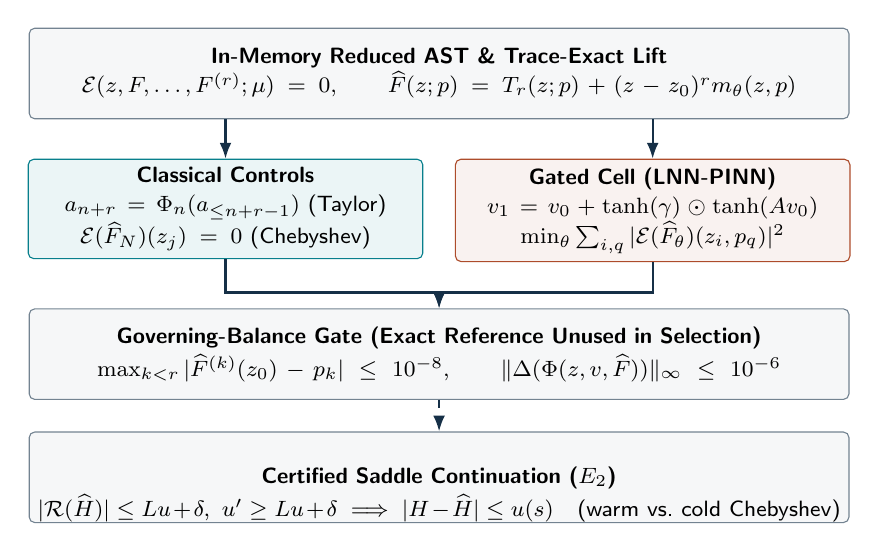
\begin{tikzpicture}[font=\sffamily\footnotesize,
  box/.style={draw=Ink!60,fill=Ink!4,rounded corners=2pt,align=center,text width=48mm,minimum height=11.5mm,inner sep=3pt},
  classical/.style={box,draw=Teal,fill=Teal!8},
  learn/.style={box,draw=Clay,fill=Clay!7},
  edge/.style={-{Latex[length=2mm]},draw=Ink,thick}]
\node[box,text width=102mm] (freeze)
  {\textbf{In-Memory Reduced AST \& Trace-Exact Lift}\\[1pt]
   $\mathcal E(z,F,\dots,F^{(r)};\mu)=0,\qquad \widehat F(z;p)=T_r(z;p)+(z-z_0)^r m_\theta(z,p)$};
\node[classical,below left=5mm and 2mm of freeze.south] (base)
  {\textbf{Classical Controls}\\[1pt]
   $a_{n+r}=\Phi_n(a_{\le n+r-1})$ (Taylor)\\
   $\mathcal E(\widehat F_N)(z_j)=0$ (Chebyshev)};
\node[learn,below right=5mm and 2mm of freeze.south] (nn)
  {\textbf{Gated Cell (LNN-PINN)}\\[1pt]
   $v_1=v_0+\tanh(\gamma)\odot\tanh(Av_0)$\\
   $\min_\theta\sum_{i,q}|\mathcal E(\widehat F_\theta)(z_i,p_q)|^2$};
\node[box,text width=102mm,below=24mm of freeze.south] (check)
  {\textbf{Governing-Balance Gate (Exact Reference Unused in Selection)}\\[1pt]
   $\max_{k<r}|\widehat F^{(k)}(z_0)-p_k|\le 10^{-8},\qquad \|\Delta(\Phi(z,v,\widehat F))\|_\infty\le 10^{-6}$};
\node[box,text width=102mm,below=4mm of check,text depth=0.3ex] (future)
  {\textbf{Certified Saddle Continuation ($E_2$)}\\[1pt]
   $|\mathcal R(\widehat H)|\le L u+\delta,\ u'\ge L u+\delta\implies |H-\widehat H|\le u(s)\quad\text{(warm vs.\ cold Chebyshev)}$};
\draw[edge] (freeze.south -| base.north) -- (base.north);
\draw[edge] (freeze.south -| nn.north) -- (nn.north);
\draw[edge] (base.south) |- ([yshift=2mm]check.north) -- (check.north);
\draw[edge] (nn.south) |- ([yshift=2mm]check.north) -- (check.north);
\draw[edge,dashed] (check)--(future);
\end{tikzpicture}
\end{document}
